\apendice{Anexo de sostenibilización curricular}

\section{Introducción}

El 25 de septiembre de 2015 se desarrolló un plan de acción por parte de la Asamblea General de Naciones Unidas a favor de erradicar la pobreza, proteger el planeta y asegurar la prosperidad y la paz universal. Este plan consta de 17 Objetivos de Desarrollo Sostenible (ODS) ~\cite{PaMuReEs24} los cuales se pueden observar en la figura \ref{fig:ODS}.

\begin{figure}[h]
    \centering
    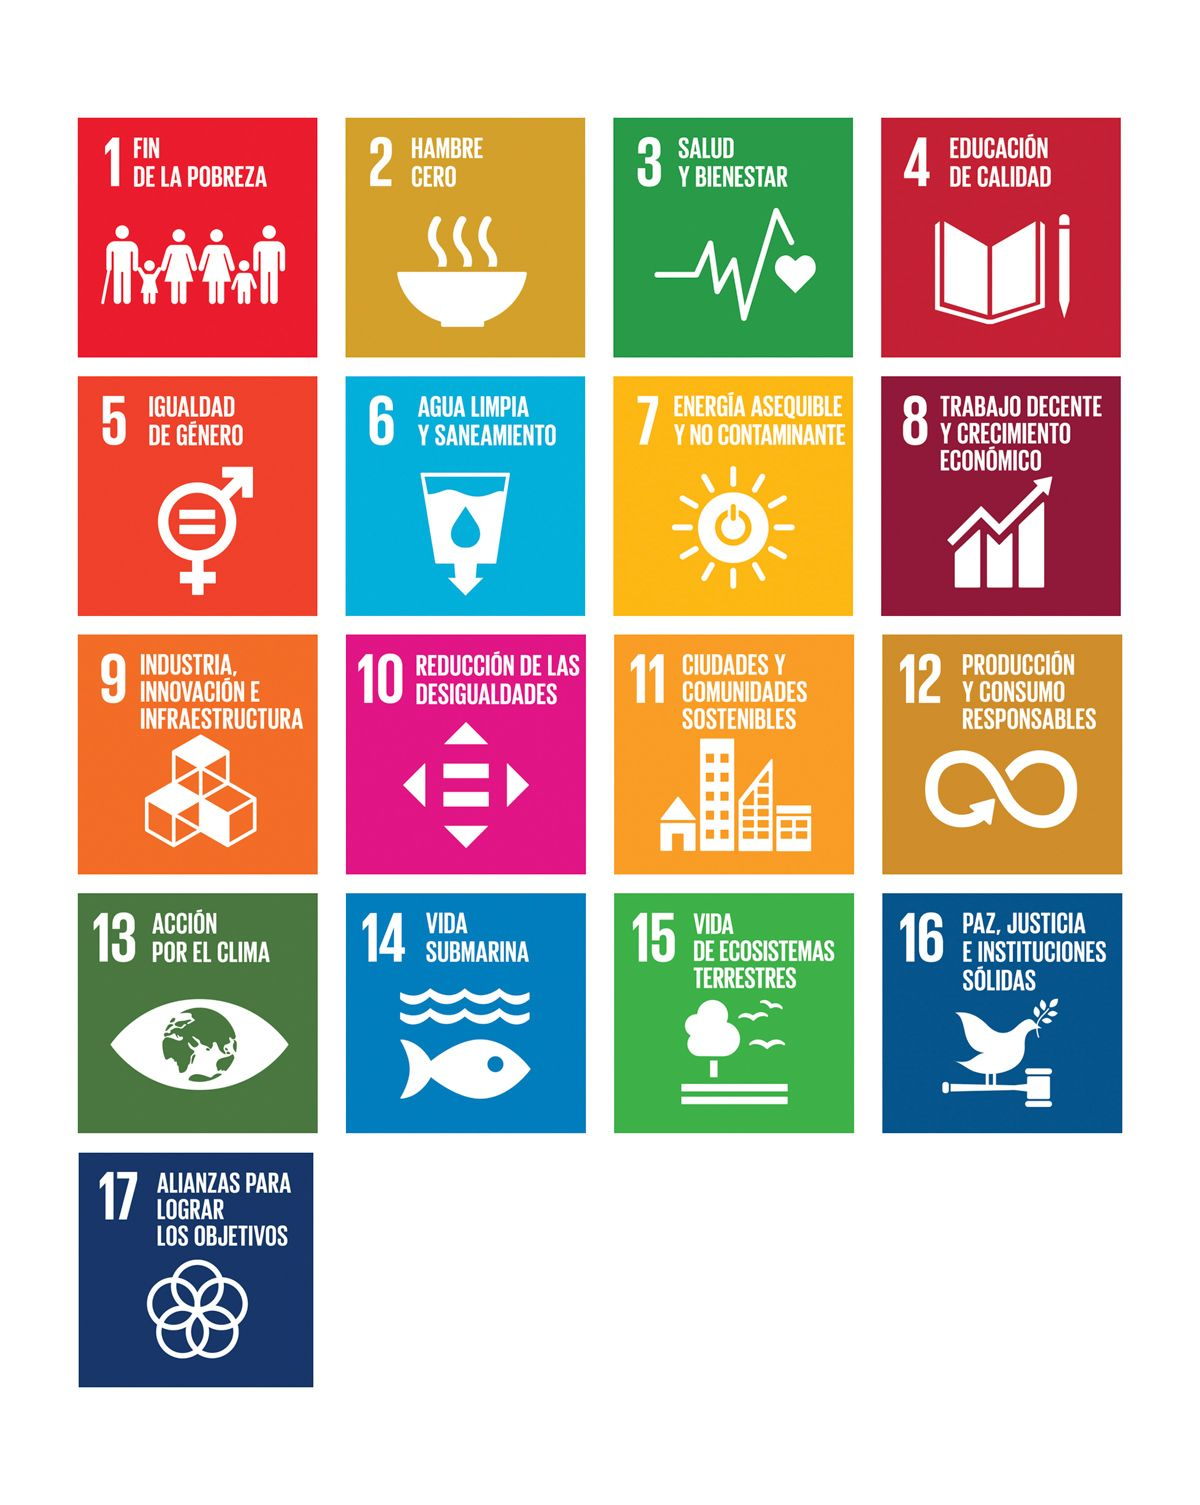
\includegraphics[width=0.99\textwidth]{img/ODS.jpg}
    \caption{ODS Objetivos de Desarrollo Sostenible.~\cite{openbank24} }
    \label{fig:ODS}
\end{figure}
\FloatBarrier

Como ya se ha comentado en otros apartados, el principal objetivo de este trabajo es la obtención de un diagnóstico más rápido, preciso y eficiente. Al margen de todos los beneficios que se pueden conseguir con esto a nivel humano reduciendo la mortalidad por neumonía y mejorando la calidad de vida de los pacientes, también se pueden obtener beneficios a nivel de sostenibilidad y medio ambiente. Ya que, con diagnósticos precisos desde un inicio, se reduce la necesidad de realizar pruebas adicionales para confirmar el diagnóstico, ahorrando tiempo y recursos. Además, también se busca reducir la desigualdad en el acceso a atención médica de calidad a nivel mundial proporcionando una herramienta accesible y eficiente, mejorando así los resultados de salud y promoviendo la equidad global en la atención médica.

Por lo tanto, este trabajo se puede relacionar principalmente con dos de los ODS.

En primer lugar, el\textbf{ ODS 3: ``Salud y bienestar''}, el cual, busca garantizar una vida sana y promover el bienestar para todos en todas las edades ~\cite{ObDeSoSalud24}. Algunas de sus metas son:
\begin{itemize}
    \item \textit{\textbf{ODS 3.2:}  ``Para 2030, \textbf{poner fin a las muertes evitables de recién nacidos y de niños menores de 5 años}, logrando que todos los países intenten reducir la mortalidad neonatal al menos hasta 12 por cada 1.000 nacidos vivos, y la mortalidad de niños menores de 5 años al menos hasta 25 por cada 1.000 nacidos vivos''} ~\cite{ObDeSoSalud24}.

    Tal y como se ha comentado en la memoria, la neumonía es una de las principales causas de muerte en niños menores de cinco años en muchas partes del mundo. Por lo que, con un diagnóstico más preciso y eficiente, se puede ayudar a reducir la mortalidad infantil.
    
    \item \textit{\textbf{ODS 3.3:}  ``Para 2030, poner fin a las epidemias del SIDA, la tuberculosis, la malaria y las enfermedades tropicales desatendidas y combatir la hepatitis, las enfermedades transmitidas por el agua y otras \textbf{enfermedades transmisibles''}} ~\cite{ObDeSoSalud24}. 
    
    La neumonía puede ser una enfermedad muy contagiosa. Por lo que, con un diagnóstico temprano y preciso se puede ayudar a prevenir la propagación y manejar mejor los brotes.

    \item \textit{\textbf{ODS 3.8:}  ``Lograr la \textbf{cobertura sanitaria universal}, en particular la protección contra los riesgos financieros, el \textbf{acceso a servicios de salud esenciales de calidad} y el acceso a medicamentos y vacunas seguros, eficaces, asequibles y de calidad para todos''} ~\cite{ObDeSoSalud24}.

    Este trabajo busca el acceso a una atención médica de calidad a nivel mundial permitiendo que hospitales con recursos limitados puedan acceder a herramientas de diagnóstico avanzadas.

    \item \textit{\textbf{ODS 3.b:}  \textbf{``Apoyar las actividades de investigación y desarrollo de vacunas y medicamentos para las enfermedades transmisibles y no transmisibles} que afectan primordialmente a los países en desarrollo y facilitar el acceso a medicamentos y vacunas esenciales asequibles de conformidad con la Declaración de Doha relativa al Acuerdo sobre los ADPIC y la Salud Pública, en la que se afirma el derecho de los países en desarrollo a utilizar al máximo las disposiciones del Acuerdo sobre los Aspectos de los Derechos de Propiedad Intelectual Relacionados con el Comercio en lo relativo a la flexibilidad para proteger la salud pública y, en particular, proporcionar acceso a los medicamentos para todos''} ~\cite{ObDeSoSalud24}.

    Aunque este trabajo no está directamente enfocado a las vacunas o los medicamentos, sí que fomenta la innovación tecnológica en el diagnóstico médico, lo que promueve grandes beneficios en el ámbito de la salud pública.

    \item \textit{\textbf{ODS 3.d:}  ``Reforzar la capacidad de todos los países, en particular los países en desarrollo, en materia de alerta temprana, reducción de riesgos y \textbf{gestión de los riesgos para la salud nacional y mundial}''} ~\cite{ObDeSoSalud24}.

    Este trabajo busca un rápido diagnóstico de la neumonía, lo que ayuda a reducir riesgos de salud derivados de un mal diagnóstico o un diagnóstico tardío a nivel mundial. 
\end{itemize}

En segundo lugar, este trabajo se puede relacionar con el \textbf{ODS 9: ``Industria, innovación e infraestructuras''} cuyo objetivo consiste en construir infraestructuras resilientes, promover la industrialización sostenible y fomentar la innovación ~\cite{ObDeSoInfraestructura24}. Algunas de sus metas son:
\begin{itemize}
    \item \textit{\textbf{ODS 9.1:} ``Desarrollar infraestructuras fiables, sostenibles, resilientes y de calidad, incluidas infraestructuras regionales y transfronterizas, para apoyar el desarrollo económico y el \textbf{bienestar humano}, haciendo especial hincapié en el acceso asequible y equitativo para todos''} ~\cite{ObDeSoInfraestructura24}.

    La implementación de una red neuronal para el diagnóstico de neumonía promueve el desarrollo de infraestructuras de calidad para apoyar el bienestar humano facilitando el acceso equitativo a los servicios básicos de salud.

    \item \textit{\textbf{ODS 9.2}: ``Promover una industrialización inclusiva y sostenible y, de aquí a 2030, \textbf{aumentar significativamente la contribución de la industria al empleo} y al producto interno bruto, de acuerdo con las circunstancias nacionales, y duplicar esa contribución en los países menos adelantados''} ~\cite{ObDeSoInfraestructura24}.

    Este proyecto contribuye con la modernización e industrialización del sistema sanitario. Lo que genera nuevas oportunidades de empleo en el desarrollo y mantenimiento de sistemas de IA relacionados con la salud.

    \item \textit{\textbf{ODS 9.5:} ``\textbf{Aumentar la investigación científica y mejorar la capacidad tecnológica de los sectores industriales de todos los países}, en particular los países en desarrollo, entre otras cosas fomentando la innovación y aumentando considerablemente, de aquí a 2030, el número de personas que trabajan en investigación y desarrollo por millón de habitantes y los gastos de los sectores público y privado en investigación y desarrollo''} ~\cite{ObDeSoInfraestructura24}.

    Este proyecto, fomenta la innovación tecnológica en el ámbito médico, lo que aumenta la necesidad de contratar profesionales relacionados con la investigación y el desarrollo de la salud digital.

    \item \textit{\textbf{ODS 9.c:} ``\textbf{Aumentar significativamente el acceso a la tecnología de la información} y las comunicaciones y esforzarse por proporcionar acceso universal y asequible a Internet en los países menos adelantados de aquí a 2020''} ~\cite{ObDeSoInfraestructura24}.

    Este trabajo mejora el acceso a tecnologías de la información al facilitar la posibilidad de realizar diagnósticos remotos, de forma que, se puede incrementar la calidad médica en zonas con recursos limitados.
\end{itemize}
